\documentclass[a4paper,11pt]{article}
\usepackage[T1]{fontenc}
\usepackage[utf8]{inputenc}
\usepackage{lmodern}
\usepackage{graphicx}
\usepackage{float}
\usepackage[francais]{babel}
\usepackage{setspace}

\onehalfspacing


\title{\LARGE{Projet composants distribués}\\\bigskip \textbf{Morse Translator}}
\author{Guillaume LAROYENNE\\
Informatique et réseau,\\
ENSISA,\\
2A\\
\bigskip
\texttt{guillaume.laroyenne@uha.fr}
}
\date{\today}

\begin{document}

    \maketitle
    \vspace{2cm}
    \begin{center}
        \large{Lien vers le logiciel de gestion de versions du projet :} \texttt{https://github.com/LaroyenneG/Morse-Tranlator.git}
        \\[2cm]
        \textit{Version de java utilisée : \texttt{\underline{Open JDK 1.7.0}}}
    \end{center}

    \newpage

    \tableofcontents

    \newpage

    \section{Présentation}
    \subsection{Description}
    \paragraph{}
    Le composant "\textit{Morse Translator}" permet de réaliser des traductions de textes simples en code Morse. Il permet également de visualiser et d'écouter les messages traduits en fonction d'une amplitude et d'une vistesse souhaitée.
    \paragraph{}
    Durant la phase de traduction, un nouveau texte est créé contenant le code Morse équivalent au texte donné au composant. Un signal analogique sera également construit correspondant au signal audio du message en Morse. Néanmoins, la construction du signal et sa lecture peuvent prendre un temps conséquent. Pour éviter que ces deux fonctionnalités du composant soient bloquante, les traitements sont effectués à l'intérieur de processus léger. Pour informer d'autres composants d'une application que ces opérations sont terminées, la programmation par événement a été utilisée.\\
    Il existe donc deux événements dans l'application :
    \begin{description}
        \item[\textit{TranslateEvent}] : Événement produit lorsque le processus de traduction et de construction du signal est terminé.
        \item[\textit{EndPlayEvent}] : Événement produit lorsque le processus de lecture audio est terminé.
    \end{description}
    \paragraph{}
    Dans le cas de l'interface de démonstration, la programmation asynchrone du composant permet à l'interface de ne jamais se retrouver dans un état "bloqué" lorsqu'elle interagit avec lui. La programmation par événements permet de réaliser des actions sur d'autres composants dès lors qu'un des processus est terminé (comme ajouter le texte traduit à une \textit{JTextArea} ou déverrouiller des boutons par exemple).


    \subsection{Aperçu}
    \begin{figure}[H]
        \begin{center}
            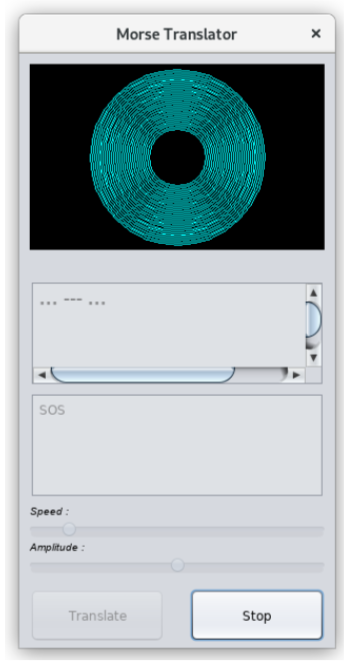
\includegraphics[scale=0.7]{descpicture.png}
            \caption{Capture d'écran de l'application de test du composant}
            \label{Capture d'écran de l'application de test du composant}
        \end{center}
    \end{figure}

    \begin{figure}[H]
        \begin{center}
            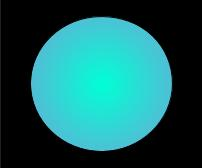
\includegraphics[scale=1]{comdescpicture.jpg}
            \caption{Interface graphique du composant}
            \label{Interface graphique du composant}
        \end{center}
    \end{figure}
    \subsection{Utilisation de l'interface de la démonstration}
    Pour utiliser l'interface vous devez entrer du texte dans la deuxième zone de texte. Une fois votre texte saisi vous pouvez appuyer sur le bouton "\textit{Translate}". Le code Morse correspondant apparaîtra dans la première zone de texte. Vous pourrez également écouter et visualiser le signal correspondent en cliquant sur le bouton "\textit{Play}".\\
    \textbf{Attention} si vous modifiez les paramètres d'amplitude ou de vitesse vous devrez recliquer sur le bouton "\textit{Translate}" pour régénérer le nouveau signal analogique.


    \section{Modèle UML}
    \subsection{Diagramme d'états transitions}
    \begin{figure}[H]
        \parshape1 -4cm 21cm
        \begin{center}
            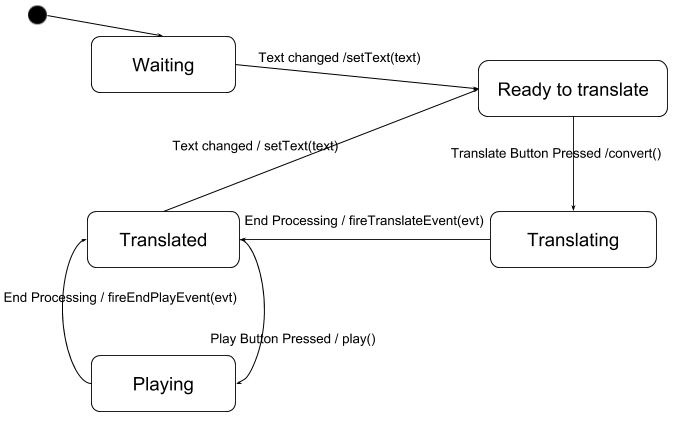
\includegraphics[scale=0.8]{etatsdiag.png}
            \caption{Diagramme d'états transitions du composant}
            \label{Diagramme d'états transitions du composant}
        \end{center}
        \parshape0
    \end{figure}
    \subsection{Diagramme des classes}
    \begin{figure}[H]
        \parshape1 -4cm 21cm
        \begin{center}
            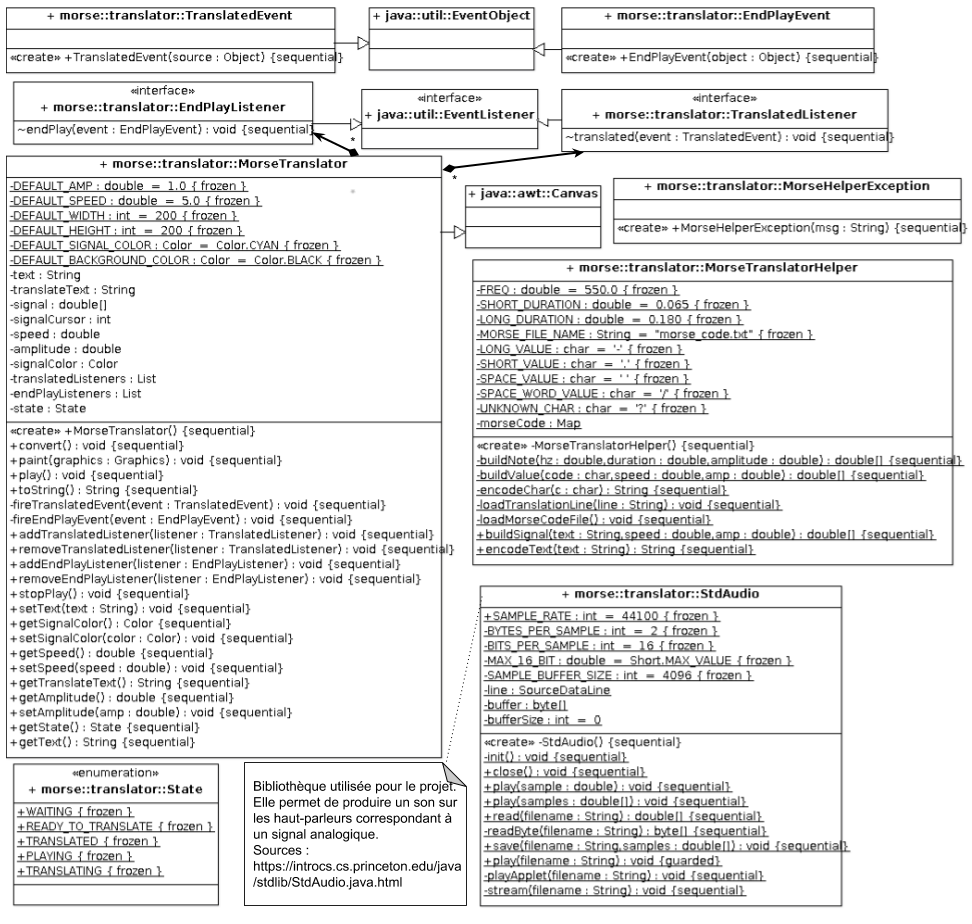
\includegraphics[scale=0.58]{classdiag.png}
            \caption{Diagramme des classes composant}
            \label{Diagramme des classes du composant}
        \end{center}
        \parshape0
    \end{figure}

\end{document}
